\setAuthor{Valter Kiisk}
\setRound{lõppvoor}
\setYear{2011}
\setNumber{G 10}
\setDifficulty{9}
\setTopic{Staatika}

\prob{Tungraud}
Joonisel on kujutatud lihtsa konstruktsiooniga tungraud,
mille keerme samm on \SI{3}{mm}. Tungrauale surub auto jõuga $F = \SI{5}{kN}$. Vaatleme hetke, millal $\alpha = \ang{40}$. Tungraua mõõtmeid vaadake jooniselt.\\
\osa Kui suure jõuga tuleb auto tõstmiseks vända käepidemele mõjuda, kui jätta
arvestamata hõõrdumine kõigi libisevate pindade vahel?\\
\osa Kui hõõre oleks ka tegelikult tühiselt väike, siis ei püsiks tungraud üleskeeratud asendis: niipea kui käepidemest lahti lasta, hakkaks see auto raskuse
mõjul pöörlema ja auto vajuks taas alla. Vastake eelmisele küsimusele eeldusel,
et hõõrdetegur on parajasti nii suur (st mitte suurem, kui hädapärast vaja),
et tungraud jääks üleskeeratud asendisse püsima.

\begin{center}
	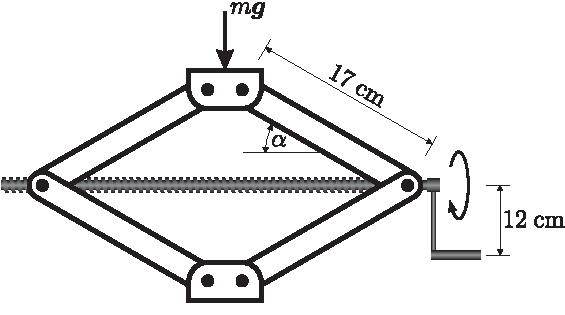
\includegraphics[scale=0.9]{2011-v3g-10-tungraud}
\end{center}

\hint
\osa Jõu määramiseks on vajalik leida, kui palju muutub tungraua kõrgus ühe vända täispöördega. Selle jaoks võib rakendada Pythagorase teoreemi tungraua pikkuse jaoks ja seda diferentseerida.\\
\osa Selleks, et tungraud oleks ilma väntamiseta hõõrdejõu tõttu tasakaalus, peab hõõrdejõud täpselt kompenseerima eelnevas alamülesandes leitud väntamiseks kuluva jõu.

\solu
\osa Olgu $a$ tungraua vertikaalne ja $b$ horisontaalne diagonaal; Pythagorase teoreemi
põhjal $a^2 + b^2 = \const$, millest diferentseerides saame
\[
2 a \Delta a+2 b \Delta b=0 \quad \Rightarrow \quad \Delta a=\frac{-b \Delta b}{a}=-\cot \alpha \Delta b.
\]
Siinjuures $\Delta a$ ja $\Delta b$ on tungraua kõrguse ja laiuse väikesed muutused. Vändaga ühe
täispöörde tegemisel $\Delta b = \SI{-3}{mm}$. Võrrutades tehtud töö $2\pi lF_k$ (kus $l$ on vända
pikkus) potentsiaalse energia muuduga $F\Delta a$, saame
\[
F_{k} =\frac{F \cot \alpha \Delta b}{2 \pi l} \approx \SI{24}{N}.
\]

\vspace{0.5\baselineskip}

\emph{Alternatiivne lahendus}

Kui vändale rakendatakse pöördemomenti $M$, siis keerates seda
väikese nurga $\Delta\Phi$ võrra tehakse tööd $M\Delta\Phi$. Kuivõrd hõõrdumine puudub, siis see
töö peab olema sama mis $F\Delta H$, kus $\Delta H$ on tungraua kõrguse muutus. Niisiis
\[
M=F \frac{d H}{d \phi}=F \times \frac{d H}{d \alpha} \times \frac{d \alpha}{d L} \times \frac{d L}{d \phi},
\]
kus $L$ on tungraua äärmiste šarniirsete kinnituste vahekaugus. Ilmselt $H = 2a \sin\alpha$,
kus $a = \SI{17}{cm}$. Seega $\D H/\D\alpha = 2a \cos\alpha$. Teiselt poolt, $L = 2a \cos\alpha$, millest $\D L/\D\alpha =
-2a \sin\alpha$. Vända üks täispööre tingib $L$ muutuse kruvikeerme sammu $h$ võrra: $\Delta L =
-(\Delta\Phi/2\pi)h$. Kokkuvõttes
\[
M=F \times(2 a \cos \alpha) \times \frac{1}{-2 a \sin \alpha} \times \frac{-h}{2 \pi}=\frac{F h \cot \alpha}{2 \pi}.
\]
Tähistades vända õla pikkuse $l$, saame avaldada otsitava jõu:
\[
F_{k}=\frac{M}{l}=\frac{F h \cot \alpha}{2 \pi l} \approx \SI{24}{N}.
\]
\osa Kui hõõrdumist ei ole, siis läheb vändast pööramisel tehtav töö puhtalt auto
potentsiaalse energia kasvatamiseks. Kui hõõrdumine on olemas tekstis kirjeldatud
määral, siis vastupidises suunas pööramisel ei ole jõudu peaaegu vaja rakendada
(tungraud püsib libisemise piiri peal) ja seega on potentsiaalse energia muut oma
moodulilt võrdne hõõrdejõudude tööga. Kui vändata päripidi (auto kergitamiseks),
siis hõõrdejõu töö ei muutu (võrreldes sama nurga võrra vastupidi pööramisega) ja
on seetõttu endiselt võrdne potentsiaalse energia muuduga. Niisiis tuleb võrreldes
hõõrdevaba pööramisega sooritada kaks korda suuremat tööd, st rakendatav jõud
peab olema täpselt kaks korda suurem, kui esimeses osas. Seega $F_1 = 2F = \SI{48}{N}$.
\probend